\section{Konzept}
Ausgehend von unseren Rechercheergebnissen haben wir unseren Fuchsjagd-Sender
folgendermaßen konzipiert.
\subsection{Versorgung}
\begin{figure}[H]
    \centering
    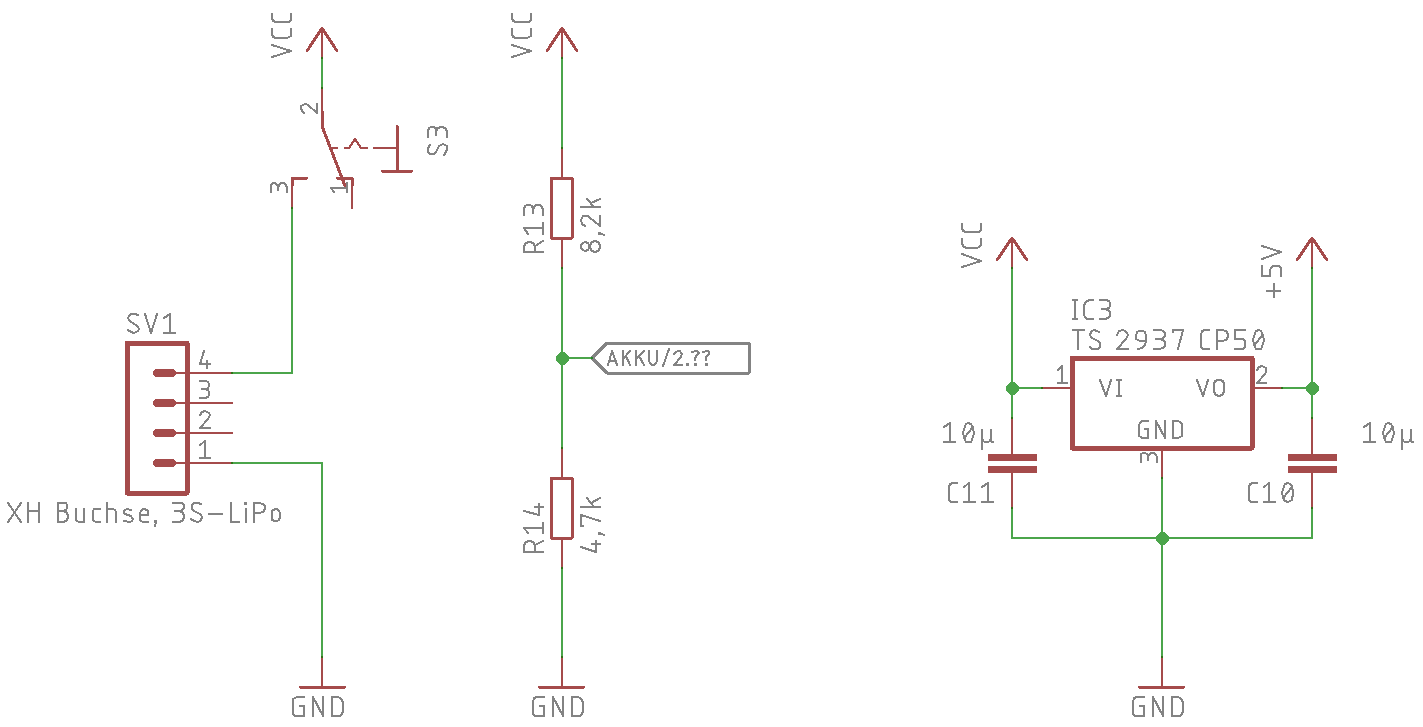
\includegraphics{res/Versorgung.png}
    \caption{Versorgung der Platine}
\end{figure}
Die Platine wird über einen dreizelligen Lithium-Ionen-Akku mit einer üblichen Nennspannung
von $11,1$V betrieben. Da unter anderem der Mikrocontroller nur mit $5$V versorgt
werden kann, nutzen wie einen Linearregler, der zusätzlich zu $12$V Schiene eine
$5$V Schiene erzeugt.